\documentclass[12pt]{article}
\usepackage{amsmath}
\usepackage{gensymb}
\usepackage{float}
\usepackage{graphicx}
\usepackage{graphics}
\graphicspath{{/storage/self/primary/Download/latexnew/fig}}
\graphicspath{{/storage/self/primary/Download/latexnew/table}}
\let\vec\mathbf
\providecommand{\brak}[1]{\ensuremath{\left(#1\right)}}
\begin{document}
\title{\textbf{VECTOR}}
\date{}
\maketitle
\textbf{Question :} Construct a triangle $APB$ in which $BC = 7cm$,$\angle B = 75\degree$ and $AB+AC = 13cm$.

\textbf{Figure :}
\begin{figure}[H]
    \centering
          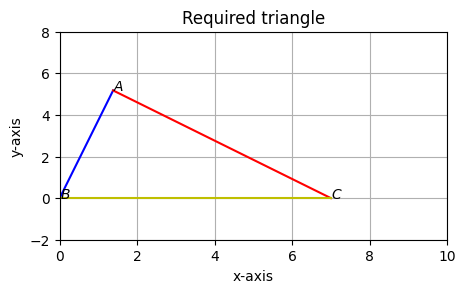
\includegraphics[width=\columnwidth]{fig/2.png}
    \caption{}
    \label{fig:fig:1}
\end{figure}

\textbf{Solution :}
\begin{table}[H]
    \centering
       \begin{tabular}{|c|c|c|}
    \hline
    \textbf{Input Parameters} &\textbf{Description} &\textbf{Value} \\
    \hline
     $\vec{O}$& Center(at origin)&$\vec{0}$\\
     \hline
 $r$ & Radius &1\\
 \hline
 $\theta$&-&$100\degree$\\
 \hline
 $\alpha$&-&$165.4\degree$\\
 \hline
 $\beta$&-&$5\degree$\\
 \hline
  \end{tabular}

    \caption{Table of input parameters}
    \label{tab:tab:1}
\end{table} 
\begin{table}[H]
    \centering
    \begin{tabular}{|c|c|c|}
    \hline
        \textbf{Output Parameters} &\textbf{Description} &\textbf{Value} \\
\hline
          $\vec{Q}$ & Point &$\myvec{\cos{\theta_1}\\\sin{\theta_1}}$\\
          \hline
          $\vec{P}$ & Point &$\myvec{\cos{\theta_2}\\\sin{\theta_2}}$ \\
         \hline
          $\vec{R}$ & Point &$\myvec{\cos{\theta_3}\\sin{\theta_3}}$ \\
         \hline
    \end{tabular}


  \caption{Table of output parameters}
    \label{tab:tab:2}
\end{table}


From appendix,
\begin{align}
    c&=\frac{k^2-a^2}{2\brak{k-a\cos{\theta}}}\\
    &=\frac{240}{52-7\sqrt{6}+7\sqrt{2}}
    \end{align}
Therefore,
\begin{align}
    \Vec{A}&=c\begin{bmatrix}
        \cos{\theta}\\\sin{\theta}
    \end{bmatrix}\\
    &=\frac{240}{52-7\sqrt{6}+7\sqrt{2}}\begin{bmatrix}
        \cos{75\degree}\\\sin{75\degree}
    \end{bmatrix}\\
    &=\begin{bmatrix}
        1.388\\5.18
    \end{bmatrix}\\
\end{align}
\end{document}


\end{document}
